%%%%%%%%%%%%%%%%%%%%%%%%%%%%%%%%%%%%%%%%%%%%%%%%%%%%%%%%%%%%%%%%%%%%%%%%%%%%%%%%%%%%%%%%%%%%%%%%%%%%%%%%%%%%
\section{Data Structure for Fast Partial Matching}\label{sec:acc}

At runtime, the user sketches a desired part. The system rapidly searches the database to find parts matching the sketch. We support searching for arbitrarily shaped parts, not just those matching a ``standard'' presegmentation. Hence, we must process each database shape on the fly, identifying which section of the shape matches the sketch. This requires an extremely fast 2D-3D partial matching method.

To compare a 2D sketch to a larger 3D shape, we have two choices: (a) to infer a 3D proxy from the sketch \cite{Igarashi:1999:TSI:311535.311602} and match it to the shape, or (b) to compare the sketch to the 2D contours of the shape. We choose to do the latter for three reasons: (i) because it avoids the inherent ambiguity in inferring 3D shape from a 2D outline; (ii) because partial matching in 3D is significantly more expensive; and (iii) because the 2D sketch reflects the user's direct intent, which may be distorted when converting to 3D.

Therefore, we perform 2D partial matching between the sketch and multi-view projections of database shapes. In the offline phase, we render and store boundary contours of each database shape from a large number of camera views. Then, the problem reduces to matching the sketch to a section of one of these exemplar contours.

\begin{figure}[t]\centering
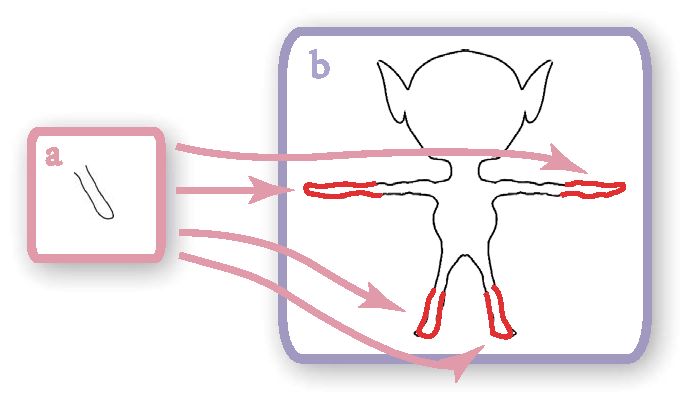
\includegraphics[width=0.85\linewidth]{./Material/CtourMatch.pdf}
\caption{A single contour may match a query contour in more than one section. The shape contour (b) matches the query contour (a) in four different sections (marked in red).}\label{fig:CtourMatch}
\end{figure}

It is a significant challenge to quickly search the huge set of exemplar contours for sections that match the sketch. Existing algorithms such as partitioning trees~\cite{scalablenearestmujapami2014}, hashing~\cite{nearoptimalandoniacm2008}, and $k$-nearest neighbor graphs~\cite{scalableknnjingwangcvpr2012} are designed for global, not partial matches.

To rapidly find database shapes whose contours match the sketch, we propose a new data structure: the {\em Randomized Compound $k$-Nearest Neighbors Graph} ({\RCKNNG}). The {\RCKNNG} has as its vertices all rendered contours of all database shapes. In a standard $k$-nearest neighbor graph~\cite{scalableknnjingwangcvpr2012}, each contour would be connected to its $k$ most similar neighbors. This information is used to quickly retrieve new matches once an initial positive match is found.

In our partial matching scenario, however, a single contour may match a query contour in more than one section, as illustrated in Figure \ref{fig:CtourMatch}. To reflect this, the {\RCKNNG} allows a contour to be connected to several different sets of $k$ neighbors. Each such set corresponds to a different matched section. Thus, from a partial match in one shape, we can quickly find several other partial matches with similar geometry in other shapes.

\begin{figure}[t]\centering
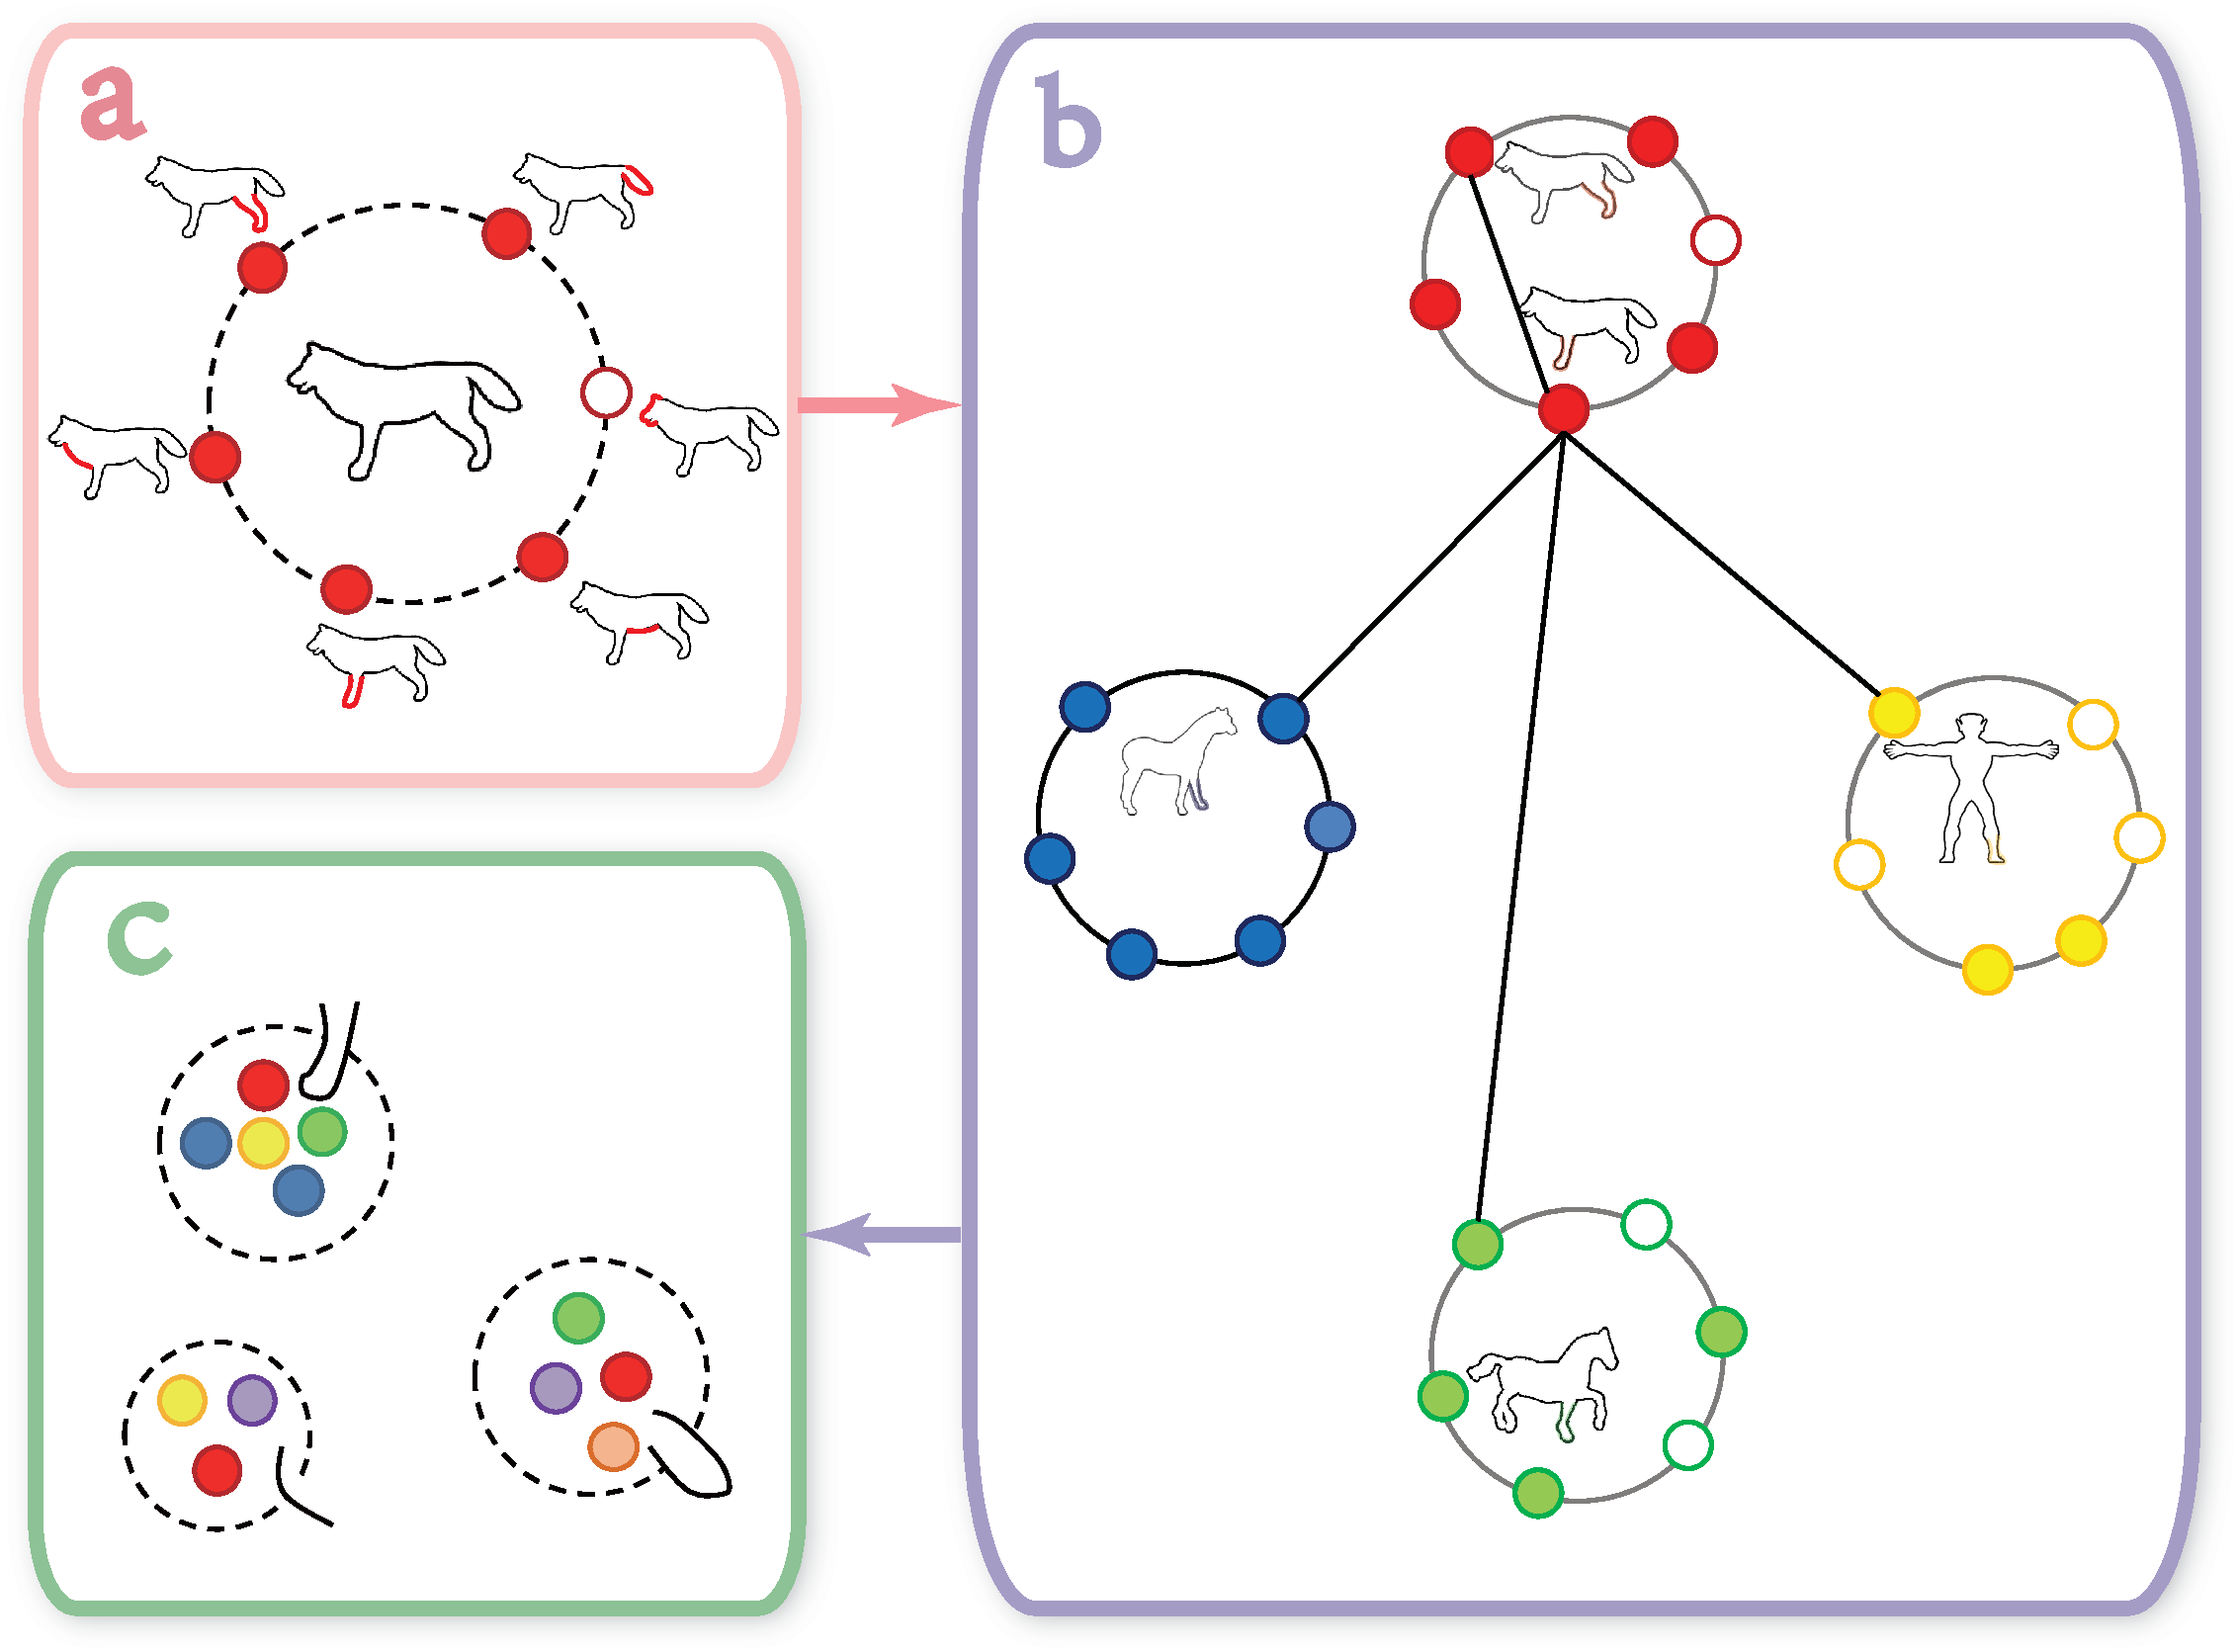
\includegraphics[width=1.0\linewidth]{./Material/KNN.pdf}
\caption{Illustration of our randomized compound $k$NN graph. In this figure, a solid circle represents a valid section and a dashed circle represents an invalid one. Given a contour (taken as a node of our randomized compound $k$NN graph), we first generate several sections (a). Then, we find the nearest neighbors for each section and establish edges between the parent contours of these sections (b). Finally, we find valid sections and cluster them (c).}\label{fig:KNN}
\end{figure}

\paragraph*{Construction of the {\RCKNNG}.} Direct construction of the compound $k$NN graph by exhaustively comparing all possible sections of all pairs of contours is prohibitively expensive. Instead, we choose to approximate the graph with a double-random strategy:
%
\begin{enumerate}
  \item We first generate $n$ sections (we use $n=6$ in our experiments) from each contour at each scale (Figure \ref{fig:KNN} (a)). A scale level comprises uniformly spaced points along the contour: a higher level has smaller spacing and hence a larger overall number of points. Our levels place $50$, $150$ and $250$ points along the contour respectively.

To generate a section, we randomly choose an uncovered point with a probability $p$ proportional to its curvature $c$ and distance $d$ to the nearest point covered by other sections: $p \propto c \cdot d$. The section then covers \st{$m = 20$} \hl{$m = 21$} consecutive points with the selected point at the center.

  \item We adopt a multiple random divide-and-conquer strategy~\cite{scalableknnjingwangcvpr2012} to construct a $k$NN graph of all the sections (Figure \ref{fig:KNN} (b)).
\end{enumerate}
%
We collect all ``valid'' sections into a global list. A section is considered valid when the distance (which will be defined in Section \ref{subsec:CtourDesc}) between it and each of its $k$ nearest neighbors is below a threshold $\varepsilon=0.85$. After that, we cluster the \hl{global} list to get a sparse set of sections (the cluster centers) which will be used as seed points for queries (Figure \ref{fig:KNN} (c)). \hl{The clustering is based on the same distance defined in Section } \ref{subsec:CtourDesc}. The number of clusters is empirically set to $1708$.
%
